% !TeX root = main.tex
\lecture{12}{Tue 03 Feb 2026 11:00}{Special Relativity IV: More Space-Time}

Recap from last lecture:
\begin{itemize}
    \item Lorentz Transformations for space and time.
    \item Lorentz Transformations for velocity/velocity addition.
    \item A Lorentz Invariant:
    The space-time interval is invariant across frames of reference:
    \[
        \delta S^2 = c^2 \Delta t^2 - \Delta r^2
    \]
\end{itemize}

In this lecture:
\begin{itemize}
    \item Minkowski space and causality.
    \item Relativistic energy and momentum.
\end{itemize}

\section{Space-Time Invariance}
Last lecture we showed that:
\[
    c^2 \Delta t^2 - \Delta r^2 = c^2 \Delta t^{\prime 2} - \Delta r^{\prime 2} = \quad (= 0 \text{ for light})
\]

And we define the space-time interval $\Delta s$ as $\Delta S^2 = c^2 \Delta t^2 - r^2$. There is some relationship between space and time that keeps this quantity constant across frames. What does this quantity actually \emph{mean}, however?

In a 3D set of axes, we have:
\[
    \Delta r^2 = \Delta x^2 + \Delta y^2 + \Delta z^2
\]

And we have defined:
\[
    \Delta s^2 = c^2 \Delta t^2 - \Delta r^2 = c^2 \Delta t^2 - \left(\Delta x^2 + \Delta y^2 + \Delta z^2\right)
\]

This looks almost like a 4D space (where one axis is time), but with some strange negative signs appearing? We don't have the equipment yet to properly understand the negative signs, but can be in future courses.

\section{Minkowski Space (Space-Time Diagrams)}
In 2D, we consider one spatial coordinate and one time coordinate, where the $x$ axis represents our spatial coordinate and the vertical axis is given by $ct$.

Consider some kind of light-emitting event happening at the origin. This light travels at a fixed speed, so we end up with the path of light at 45 degrees on this space-time diagram:

\begin{figure}[H]
    \centering
    
\includegraphics[width=0.5\textwidth]{figures/lec12-01.png}
     \caption{}
\end{figure}

These are given by the lines $c^2 t^2 = \pm x^2$ and are called ``light cones'', as they form cones in higher dimensions. The positive velocity axis is called the ``future cone'', the path taken by light emerging from event A. The negative velocity axis is called the ``past cone'', and represents the path taken by light emerging at A.

\begin{figure}[H]
    \centering
    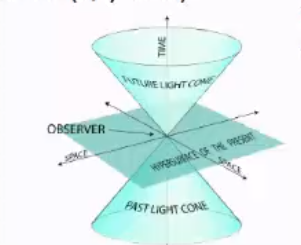
\includegraphics[width=0.75\textwidth]{figures/lec12-02.png}
     \caption{Light cones in a 3D space (two spatial, one velocity)}
\end{figure}

Inside the future cone, events may be caused by the event happening at A. Things travelling at a velocity $<c$ can reach them.

The region inside the past cone gives regions in spacetime where events could have caused A. 

Events outside the two cones cannot influence, nor can they be influenced by A. They cannot be causally connected in any way to the event at A.

We now have two events. A is defined as before, and a new event B separated from A by distance $\Delta \underline{r}$ and time $\Delta t$.

What is the condition that B lies within the light cone given by A? We require:
\[
    | \Delta \underline{r} | \leq c | \Delta t |
\]

Or in invariant form:
\[
    \Delta S^2 = c^2 \Delta t^2 - \Delta r^2 \geq 0
\]

We call $\Delta S$ the space-time interval, or invariant distance.

There are three possible cases:
\begin{itemize}
    \item $\Delta S^2 > 0$, ``time-like intervals''. This is where $| \Delta \underline{r} | \leq c | \Delta t |$ and B is inside A-s light cone. $\Delta S \in \R$. Here, a signal can pass between A and B and the two events may be causally connected (where A causes B).
    \item $\Delta S^2 = 0$. Here, $| \Delta \underline{r} | = c | \Delta t |$. This is where B sits on A's light cone, and A/B may be causally connected. A signal can only travel between the two events if the signal is at velocity $c$. This is called a ``light-like interval''
    \item $\Delta S^2 < 0$, ``space-like intervals''. This is where $| \Delta \underline{r} | > c | \Delta t |$. $\Delta S = \sqrt{c^2 \Delta t^2 - \Delta r^2} \in i\R$. No signal can pass between A and B, not even light. No causal connection is possible.
\end{itemize}

\section{Causality and Time Order}
It is possible for observers in two different frames to disagree on the order in which events have taken place. If we have two events with $t_1, t_2$ in $\Sigma$ and $t_1^\prime$, $t_2^\prime$ in $\Sigma^\prime$, there are possible cases where:
\begin{itemize}
    \item $t_2 > t_1$.
    \item $t_1^\prime > t_2^\prime$.
\end{itemize}

This may seem uncomfortable - does this cause a breakdown in causality?

Suppose we have a frame $\Sigma$ with two events, $(x_1, t_1)$, $(x_2, t_2)$, such that $\Delta t = t_2 - t_1 > 0$.

Frame $\Sigma^\prime$ moves with speed $v$ relative to $\Sigma$ and in $\Sigma^\prime$ the same two events have coordinates $(x_1^\prime, t_1^\prime)$ and $(x_2^\prime, t_2^\prime)$. For the observers to disagree on causality, we have $\Delta t^\prime t_2^\prime - t_1^\prime < 0$. We begin by applying the Lorentz Transformation to $\Delta t^\prime$:
\[
    \Delta t^\prime = \gamma \left(t_2 - \frac{v}{c^2} x_2\right) - \gamma \left(t_1 - \frac{v}{c^2} x_1\right) < 0
\]
\[
    \implies \gamma(t_2 - t_1) + \frac{\gamma v}{c^2} \left(-x_2 + x_1\right) <0
\]
\[
    \Delta t - \frac{v}{c^2} \Delta x < 0
\]

I.e. $\Delta t < \frac{v}{c^2} \Delta x$ or $c \Delta t < \frac{v}{c} \Delta x$. We know that $v/c < 1$, hence $c \Delta t < \Delta x$. This means that:
\[
    \Delta S = \sqrt{c^2 \Delta t^2 - \Delta x^2}
\]

Which is the square root of a negative number, hence this gives a space-like interval. This means that while we can define two points in space-time where two observers will disagree about their order, the space-time invariant is imaginary hence these events cannot be causally linked. This means that observers disagreeing on event order does not break causality.

